\documentclass[11pt]{article}
\usepackage[margin=1in]{geometry}
\usepackage{authblk}
\usepackage{amsmath,amssymb,graphicx,booktabs}
\usepackage[hidelinks]{hyperref}
\usepackage{orcidlink}
\newcommand{\ms}{\overline{\mathrm{MS}}}
\emergencystretch=1.5em
\begin{document}

\title{The inverse branch of the compact family cycle:\\ down-type quark masses from waveform-carried partners}

\author{Andrew M. Brilliant\,\orcidlink{0009-0004-8024-5442}}
\affil{Applied Dynamics Research, Sapporo, Japan; ab@ad-research.org}


\date{\today}

\maketitle

\begin{abstract}
The charged-lepton mass relation and the recently reported inverse down-quark
sum rule are shown to be one cone condition read in two coordinates of a single
compact-cycle construction. An exact circulant fit diagnoses which coordinate
each sector uses: the self-dual condition $k=1$ holds for the leptons directly
($k=1.00000\pm0.00001$, pole masses) and for the down triple inversely
($k=1.001\pm0.002$ at $2$\,GeV), while the up triple satisfies neither
($k=1.24$/$1.32$). A Monte Carlo budget under stated priors prices the joint
two-cone structure at $6.3\times10^{-6}$ of null universes (sharp threshold;
$3\times10^{-5}$ convolved with input uncertainties); every researcher freedom
exercised after the data were inspected is restored and priced, and the rarity
survives each freedom singly, failing only when all are granted at once
($\sim0.5$, quoted as-is). A universal-seesaw realization, in which heavy
vectorlike partners carry the waveform, trades the coupling postulate for a
standard assumption about particle content and excludes its own most economical
version by direct searches. Self-duality fixes $m_s$ from $(m_d, m_b)$ as a
consistency condition at present data ($-0.2\sigma$ from PDG 2026,
$-0.4\sigma$ from FLAG); future lattice precision makes this a decisive test.
Around the same lepton-sum scale the construction registers five of six quark
masses: the light cascade at $\mu_\star$, and the heavy pair through the
pre-registered anchored form $m_b(m_b) = \mu_\star/2\alpha$ ($+0.9\sigma$) with
the charm as its mirror image ($-0.7\sigma$); cross-sector relations enter as
outputs, not premises. No fit parameter is introduced into the mass relations;
the seesaw realization adds vectorlike fields and a free common scale, which
are not counted as fit parameters because they do not enter the mass
predictions.
\end{abstract}


\section{A coordinate ambiguity, and a construction that resolves it}

Any three positive masses can be organised either through their square roots or
through their inverse square roots; the two coordinates carry different physics
when a structural condition holds in one and not the other. This paper shows
that the light-fermion spectrum exhibits exactly this situation, that the two
coordinates correspond to the two coupling branches of a single recent
construction, and that a universal-seesaw realization connects them.

The structural condition in question is a constraint the charged-lepton pole
masses are observed to satisfy~\cite{Koide1982,Koide1983,PDG},
\begin{equation}
Q_\ell \equiv \frac{m_e+m_\mu+m_\tau}{\left(\sqrt{m_e}+\sqrt{m_\mu}+\sqrt{m_\tau}\right)^2}
= \frac{2}{3},
\label{eq:koide}
\end{equation}
for which Shulga~\cite{Shulga2026} has
proposed a mechanism: a single real amplitude on a compact internal cycle, built
from the two lowest antiperiodic modes $e^{\pm i\varphi/2}$, whose symmetric square
spans the three periodic harmonics $\{e^{i\varphi},1,e^{-i\varphi}\}$ identified
with the three families. A coherence (self-duality) condition fixes the amplitude to
\begin{equation}
Z(\varphi) = s\left[1+\sqrt{2}\cos(\varphi+\delta)\right],
\label{eq:Z}
\end{equation}
and the masses are quadratic overlaps at the three family phases,
$m_a \propto |Z(2\pi a/3)|^2$. Orthogonality of equally spaced samples gives
$\sum_a z_a = 3s$ and $\sum_a z_a^2 = 6s^2$ for \emph{any} $\delta$, hence
Eq.~(\ref{eq:koide}) exactly. A Berry dressing selects $\delta_\ell = -2/9$ and
predicts $m_\tau = 1776.97$\,MeV; the construction is explicitly restricted to
the charged leptons. Equation~(\ref{eq:koide}) holds on the measured pole
masses to one part in $10^5$, and, because the mass anomalous dimension is
flavour-blind, is built from ratios that are numerically stable under renormalisation-group running to high precision~\cite{LiMa}.

Separately, Rivero~\cite{Rivero2026} has reported that the down-type quarks satisfy
the same constant in the \emph{inverse} coordinate,
\begin{equation}
Q_d^{\,\rm inv} \equiv
\frac{m_d^{-1}+m_s^{-1}+m_b^{-1}}{\left(m_d^{-1/2}+m_s^{-1/2}+m_b^{-1/2}\right)^2}
= \frac{2}{3},
\label{eq:rivero}
\end{equation}
holding within $1\sigma$ across the perturbative range, with the deviation from
$2/3$ crossing zero in the $10$--$300$\,TeV region depending on running inputs.
The same ratio invariance renders the relation observationally near
scale-free.

This paper makes one structural observation, one empirical observation, and one
honest accounting of what remains underived.

\section{One condition, two coordinates}

The algebraic content is a single lemma (the proof is division of the two sum
rules already stated, $\sum_a z_a = 3c_0$ and $\sum_a z_a^2 = c_0^2(3+3A'^2/2)$;
the identities are machine-checked in Lean~4; repository at \url{https://github.com/AndBrilliant/inverse_branch}). Let three quantities be sampled from one cosine
at $120^\circ$ spacing, $z_a = c_0[1+A'\cos(\varphi_a+\delta)]$,
$\varphi_a = 2\pi a/3$. Then
\begin{equation}
\frac{\sum_a z_a^2}{\left(\sum_a z_a\right)^2} = \frac{1}{3}+\frac{A'^2}{6},
\end{equation}
which equals $2/3$ if and only if $A' = \sqrt{2}$, the self-dual point of Eq.~(\ref{eq:Z}). The rational value is therefore not a tuned target: it is the participation ratio forced by the orthogonality of three equally spaced samples at the self-dual amplitude, for any phase. The derivation never asks what $z$ is. Setting $z_a = \sqrt{m_a}$
yields Eq.~(\ref{eq:koide}); setting $z_a = 1/\sqrt{m_a}$ yields
Eq.~(\ref{eq:rivero}). The two relations are one cone condition read in two coordinates (geometrically, the condition places the coordinate vector at $45^\circ$ to the democratic direction~\cite{Foot}). The algebra permits both coordinates and selects neither; the
selection is physics, and it is the subject of Sec.~\ref{sec:open}.

\section{The transfer: an inverse coupling branch}
\label{sec:transfer}

Retain Shulga's construction in full (cycle, antiperiodic doublet, symmetric square, self-dual coherence) and change only the coupling of the down sector to
the family amplitude:
\begin{equation}
m_a^{(\ell)} \propto |Z_\ell(2\pi a/3)|^2,
\qquad
m_a^{(d)} \propto \frac{M_d^2}{|Z_d(2\pi a/3)|^2}.
\label{eq:branches}
\end{equation}
Then $1/\sqrt{m_a^{(d)}} \propto Z_d(2\pi a/3)$, and the same two sum rules give
Eq.~(\ref{eq:rivero}) exactly, for any down-sector phase $\delta_D$. This is the single new postulate of the paper, and it is flagged as such: the inverse branch is \emph{assumed} here, with a candidate realization, in which the assumption migrates from the coupling to the particle content, given in Sec.~\ref{sec:open}. Everything downstream (the exactness of Eq.~(\ref{eq:rivero}), its phase independence, its scale behaviour) is
inherited from the mechanism without modification (Fig.~\ref{fig:branches}).

\begin{figure}[t]
\centering
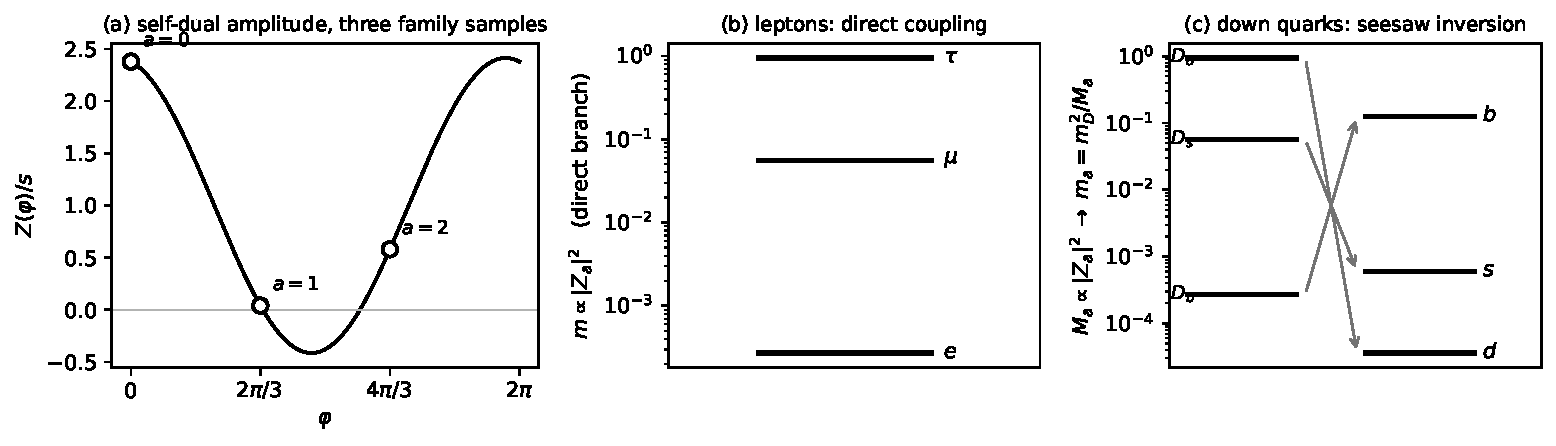
\includegraphics[width=\linewidth]{fig_branches}
\caption{The two coupling branches of one waveform. (a) The self-dual amplitude
$Z(\varphi)/s = 1+\sqrt{2}\cos(\varphi+\delta)$ at $\delta=2/9$, sampled at
the three family phases $2\pi a/3$. (b) Direct branch: charged-lepton masses as
squared overlaps, $m \propto |Z_a|^2$. (c) Inverse branch via the universal
seesaw of Sec.~\ref{sec:open}: vectorlike partner masses carry the waveform, $M_a \propto |Z_a|^2$ (levels $D_d, D_s, D_b$), and integrating them out inverts the ladder,
$m_a = m_D^2/M_a$: the heaviest partner yields the lightest quark. Both
panels share the sum rules $\sum z_a = 3s$, $\sum z_a^2 = 6s^2$, hence the
$2/3$ cone in the respective coordinate.}
\label{fig:branches}
\end{figure}


\section{The empirical structure being mechanised}
\label{sec:cascade}

The inverse branch is not proposed in a vacuum. Two companion
letters~\cite{APPB,MPLA} establish the empirical pattern this paper seeks to
connect to Shulga's cycle; we state it here for self-containment.

The Soddy completion of the lepton Descartes configuration~\cite{APPB} fixes
a companion scale $F^2 = \alpha^2\mu_\star = 95.12$\,MeV, with $\alpha \equiv
\sqrt{3/2}-1$ determined by the cone condition alone ($(1+\alpha)^{-2} = 2/3$).
This scale coincides with $m^{\overline{\rm MS}}_s(\mu_\star)$ at $+0.9\sigma$
of the printed $90\%$ interval, $+1.4\sigma$ in $1\sigma$ units (PDG 2026)
--- the largest pull in the cascade register, recorded openly; its rivalry
with the exact-self-duality value of Sec.~\ref{sec:diagnosis} is test (5). Accepting this identification, the companion
letter~\cite{MPLA} develops the cascade:
\begin{align}
m_s &= \alpha^2\,\mu_\star = 95.12\ \mathrm{MeV}, \label{eq:cascade_s}\\
m_d &= \alpha^4\,\mu_\star = 4.804\ \mathrm{MeV}, \label{eq:cascade_d}\\
m_u &= \alpha^2\sqrt{2m_e\,\mu_\star} = 2.216\ \mathrm{MeV}, \label{eq:cascade_u}
\end{align}
all at $\mu_\star$. Each rung steps by $\alpha^2$; the chain interpolates
geometrically between the lepton-sum scale $\mu_\star$ and the pair-production
threshold $2m_e$, closing the loop $\mu_\star \to m_s \to m_d \to m_u \to 2m_e
\to e \to \mu_\star$. The ratio $m_d/m_s = \alpha^2 = 5/2-\sqrt{6}$ gives,
via the leading Gatto--Sartori--Tonin relation~\cite{GST},
$\sqrt{m_d/m_s} = \alpha = 0.22474$, within $0.4\sigma$ of
$|V_{us}|$~\cite{MPLA}.

A remark on economy of description. Read as numerology, the rung forms of
Eqs.~(\ref{eq:cascade_s})--(\ref{eq:cascade_u}) need a single input --- the
measured lepton sum $\mu_\star$ --- together with the cone constant and small
integers, where a Koide-style statement of the same content requires two
measured masses to return a third. The deeper layer is the waveform: the
compact forms are the self-dual amplitude's readout at the family phases, not
an independent pattern, and they are used here as the construction's
compact register --- mechanism outputs in form, anchored to the measured
phase in value --- rather than as fitted relations or first-principles
derivations.

The geometric-mean structure $m_s^2 = \mu_\star\cdot m_d$ (equivalently,
$m_s$ is the mean proportional of $\mu_\star$ and $m_d$) was noted empirically
by Ng~\cite{Ng} in the form $m_s^2 \approx m_d\cdot m_b$, with the heavy-quark
boundary replaced here by the lepton-sum scale.

The light-sector cascade has a heavy-sector counterpart. Define
$G \equiv \sqrt{3/2}\,\mu_\star = 2306.3$\,MeV, a scale built from the cone
condition and the lepton sum. The charm--bottom pair mirrors about it:
\begin{equation}
m_c \cdot m_b = G^2 = \tfrac{3}{2}\,\mu_\star^2,
\label{eq:involution}
\end{equation}
an involution $m \mapsto G^2/m$ exchanging charm and bottom, whose fixed
point is $G$ itself. The mirror factorises into two separately registered
forms~\cite{Prereg},
\begin{equation}
m_b(m_b) = \frac{\mu_\star}{2\alpha} = 4189.4\ \mathrm{MeV},
\qquad
m_c(m_c) = 3\alpha\,\mu_\star = 1269.7\ \mathrm{MeV},
\label{eq:anchoredb}
\end{equation}
whose product is $\tfrac{3}{2}\mu_\star^2$ identically. Pulls are quoted in
$1\sigma$ units throughout this paper; the PDG 2026 quark evaluations are
printed at $90\%$\,CL ($m_b(m_b) = 4186\pm6$\,MeV,
$m_c(m_c) = 1272.9\pm4.5$\,MeV~\cite{PDG}) and are converted by the Gaussian
factor $1.645$. The anchored bottom then stands at $+0.9\sigma$ --- the
evaluation itself moved toward the frozen form, $4183 \to 4186$\,MeV, taking
the residual from $+1.5\sigma$ to $+0.9\sigma$ --- and the mirror charm,
registered conditionally as $G^2/m_b = 1270.7\pm1.1$\,MeV against the
measured bottom, at $-0.7\sigma$; the pure closed form
$3\alpha\mu_\star = 1269.7$\,MeV reads $-1.2\sigma$ in the same units and is
carried as the mirror's algebraic identity, not as the register entry. (A
one-step drift toward any frozen target carries even odds under a random
walk; the registration's content is the standing agreement at the frozen
value, not the direction of the move.) This is a second
lepton-anchored geometric-mean relation: the geometric mean of charm and
bottom is $G$, determined by $\mu_\star$ alone. Combined with the light
cascade, the construction links five of six quark masses to the single
lepton-sector input $\mu_\star$ through geometric means at both ends of the
spectrum (the top quark, which decays before hadronising and whose pole mass
is perturbatively well-defined, is not addressed here). Neither the
involution nor the light cascade is scored in the coincidence budget of
Sec.~\ref{sec:budget}, which prices only the two-cone self-duality; the
full geometric-mean structure is correspondingly rarer than the quoted
frequency, as priced in Sec.~\ref{sec:budget} (Table~\ref{tab:rungs}); we
report it there without claiming it.

\emph{What the cone condition does and does not fix.} Self-duality ($k=1$)
forces $Q = 2/3$ for every phase $\delta$, but the mass \emph{ratios} depend
on $\delta$: different phases produce different hierarchies on the same cone.
The $\alpha^2$ stepping of the cascade therefore requires both $k=1$ and the
measured phase; the cone condition alone is necessary but not sufficient.
Under the seesaw realization of Sec.~\ref{sec:open}, the light down mass at
family phase $\varphi_a$ is $m_a = m_D^2/M_a$ with
$M_a \propto |Z(2\pi a/3)|^2$, so the mass ratios inherit the waveform's
phase structure. The cascade is consistent with, and expressed in the
language of, the cone condition, but it is not derived from self-duality
alone: deriving the phase remains an open problem (Sec.~\ref{sec:open},
problem B).

\emph{Scale selection.} A running mass crosses every target inside its range
(the intermediate-value theorem applied to a continuous, monotone function),
so a match found by scanning establishes nothing: continuous scale variation
is a coincidence generator, and it is not admitted here. The comparison
scale $\mu_\star$ is not scanned; it is the lepton-sum scale, fixed by
Eq.~(\ref{eq:koide}) and the measured lepton masses before any quark
comparison is made~\cite{APPB}. The match is specific: shifting the comparison scale by $\pm5\%$ moves the cascade prediction of $m_s$ by $\sim7\sigma$ from the FLAG central value, and by $\pm10\%$ by $\sim14\sigma$; continuous scale variation is a coincidence generator and these margins show the match is not generic. A cross-scheme audit confirms this specificity: at the conventional
reference scale $2$\,GeV the cascade values miss by $>2\sigma$
(four-loop running via RunDec~\cite{CRunDec}, $\alpha_s(M_Z)=0.1180$),
and under QED-corrected lepton inputs (MS masses at $\mu_\star$ in
place of pole masses) the residual shifts by $<0.2$\,MeV, so the
cascade output is scale-locked rather than generically compatible.
The seed's specialness is functional, not only metrological: among the
lepton-derived scale prescriptions scanned in the companion analysis,
$\mu_\star = \sum m_\ell$ is the unique one at which the cascade lands on
the data, the $1\sigma$ window around it only $\pm2\%$ wide and the
next-best prescription ($m_\tau$ alone) missing by $2.3\sigma$~\cite{Prereg}.

Two remarks. First, the postulate is economical: no new field, scale, or parameter
is introduced; the branch is a discrete label. Second, it is not vacuous: the
crossed assignments miss the self-dual point decisively --- the down triple
read directly deviates by $11\%$ in the amplitude parameter
(Table~\ref{tab:k}), the lepton triple read inversely by $25\%$
($k = 1.247$).

\section{Coordinate diagnosis: self-duality selects the branch}
\label{sec:diagnosis}

Any three positive masses admit the exact circulant parametrization of
Koide, Brannen and \.{Z}enczykowski \cite{Brannen,Zen2012,Zen2013},
\begin{equation}
v_j = A\left[1+\sqrt{2}\,k\cos\!\left(\tfrac{2\pi j}{3}+\delta\right)\right],
\qquad j = 0,1,2,
\label{eq:circulant}
\end{equation}
with $v_j = \sqrt{m_j}$ (direct coordinate) or $v_j = 1/\sqrt{m_j}$ (inverse
coordinate). Three data determine $(A,k,\delta)$ exactly by discrete Fourier
inversion; no fitting is involved. The participation ratio in either coordinate is $Q = (1+k^2)/3$, so the self-dual point $k=1$ is precisely $Q = 2/3$.

Table~\ref{tab:k} gives the exact-fit $(k,\delta)$ for each sector in each
coordinate. Lepton inputs are pole masses (scheme-independent).
\emph{Down triple:} all three masses at a common $\overline{\rm MS}$ scale
$\mu = 2$\,GeV: $m_d = 4.70\pm0.07$\,MeV (PDG 2026, printed at $90\%$\,CL
and converted by $1.645$~\cite{PDG}), $m_s = 93.4\pm0.68$\,MeV (FLAG 2024,
$N_f{=}2{+}1{+}1$, $1\sigma$~\cite{FLAG}), $m_b(2\,\mathrm{GeV}) = 4970$\,MeV from
four-loop running of $m_b(m_b) = 4186\pm6$\,MeV~\cite{CRunDec}; no mixed scales.
\emph{Up triple:} $m_u = 2.16$\,MeV at $2$\,GeV, with $m_c(m_c)$ and $m_t(m_t)$
at their own scales, following the mixed-scale convention
of~\cite{Zen2012} for comparability with his published $k$ values. The
common-scale cross-check is given in Sec.~\ref{sec:diagnosis}(ii).

\begin{table}[t]
\caption{Exact circulant parameters by sector and coordinate. The self-dual condition $k=1$ holds in exactly one coordinate per cone-satisfying sector and in neither coordinate for the up triple. Uncertainties on the down-triple inverse row
are input-propagated ($m_d$ dominant for $\delta$, $m_s$ for $k$).}
\label{tab:k}

\begin{tabular}{llll}\toprule
sector & coordinate & $k$ & $\delta$ (rad) \\
\midrule
$e,\mu,\tau$ & direct  & $1.00000(1)$ & $+0.22222$ ($\simeq 2/9$) \\
$d,s,b$      & direct  & $1.115$   & $+0.1002$ \\
$d,s,b$      & inverse & $1.001\pm0.002$ & $-0.1898\pm0.0019$ \\
$u,c,t$      & direct  & $1.239$   & $+0.0769$ \\
$u,c,t$      & inverse & $1.324$   & $-0.0333$ \\
\bottomrule\end{tabular}

\end{table}

Three features of Table~\ref{tab:k} carry the paper's empirical content.

\emph{(i) The self-dual condition diagnoses the branch.} The charged leptons sit at
$k=1$ to five decimal places in the direct coordinate. The down triple sits at
$k = 1.001\pm0.002$ in the inverse coordinate (Rivero's relation restated)
while deviating by $11\%$ in the direct coordinate. \.{Z}enczykowski, working in
the direct coordinate only, reported $k_D \simeq 1.08$ and $k_U \simeq 1.25$ at
$2$\,GeV and read these as the failure of Koide's parametrization for
quarks~\cite{Zen2012}; our exact fit reproduces his values with current masses
($1.115$, $1.239$). The resolution proposed here is that the parametrization does
not fail for the down sector: it is being read in the wrong coordinate. Where
$k=1$ lives is an empirical fact, and it is the fact the mechanism's branch
structure, Eq.~(\ref{eq:branches}), encodes. The statement is stable across
input vintages: FLAG 2024, PDG 2024, and PDG 2026 central values give
$k^{\rm inv}_{dsb}$ in $[1.000, 1.002]$, and varying $m_d$ by $\pm1\sigma$
spans $[0.999, 1.003]$, consistent with the quoted input-propagated uncertainty. (Uncertainties on $(k, \delta)$ are propagated through the discrete Fourier inversion of Eq.~(\ref{eq:circulant}), taking the printed light-quark errors as $1\sigma$ --- conservative for $m_d$, whose PDG $\pm0.07$\,MeV is a $90\%$\,CL half-width and whose FLAG error is $\pm0.05$\,MeV; the threshold convolutions of Sec.~\ref{sec:budget} inherit the same choice. Under independent variation, $m_d$ dominates ($\partial k/\partial m_d \simeq -0.033$\,MeV$^{-1}$; $\partial k/\partial m_s \simeq 0.0014$), giving $\sigma_k = 0.0025$. Because FLAG determines $m_d$ and $m_s$ from the same lattice ensembles, their uncertainties are correlated; a worst-case envelope over all $\pm1\sigma$ combinations (including full positive and negative correlation) gives $|k-1| < 0.005$ in every case, with $k$ ranging from $0.998$ to $1.004$. The self-duality conclusion ($|k-1|$ compatible with zero) is robust to correlations at the $1\sigma$ level.)

\emph{(ii) The up triple satisfies neither coordinate.} $k$ deviates from unity by
$24\%$ (direct) and $32\%$ (inverse), equivalently $Q = 0.845$ and $0.918$,
consistent with Kartavtsev's published $K_u \sim 0.85$~\cite{Kartavtsev}. Within
the present framework this is an open problem, not an embarrassment: a sector with different combinatorial structure (Rivero's construction distinguishes up- and down-type sectors through different multiplet counts, $k_d=3$ vs.\ $k_u=2$~\cite{Rivero2024}) is not expected to sample the waveform as a
triplet does, and no cone form in either coordinate should hold. A
representation-theoretic computation of the up-sector participation ratio,
confronting the measured $0.845$/$0.918$, would be a decisive test; none exists. (Table~\ref{tab:k} follows the mixed-scale convention of~\cite{Zen2012} for comparability; at a true common scale, $\mu = 2$\,GeV under four-loop running, the triple reads $k^{\rm dir} \simeq 1.29$ and $k^{\rm inv} \simeq 1.32$, so the neither-coordinate conclusion is convention-independent.)

\emph{(iii) A sharp forward test.} Imposing self-duality exactly in the inverse
coordinate, Eq.~(\ref{eq:rivero}) determines any one down mass from the other two.
The binding constraint is on the strange quark:
\begin{equation}
m_s(2\,\mathrm{GeV})\big|_{\rm pred} = 92.64\ \mathrm{MeV},
\end{equation}
from $(m_d, m_b)$ input. Propagating the input uncertainties gives a theory-side error of $\pm1.6$\,MeV, dominated entirely by $m_d$
($\partial m_s/\partial m_d \simeq 23$; the $m_b$ contribution is $0.02$\,MeV, propagated from $m_b(m_b) = 4.186\pm0.006$\,GeV through four-loop running via RunDec~\cite{CRunDec}), so the single-mass comparison is $m_d$-limited: $-0.4\sigma$
combined against FLAG 2024 ($93.4\pm0.68$\,MeV~\cite{FLAG}) and $-0.2\sigma$
against PDG 2026 ($92.9\pm0.7$\,MeV). The sharp form of the same constraint is
dimensionless and renormalisation-group invariant: the parametrisation Eq.~(\ref{eq:circulant}) at $k=1$ has two free parameters $(A, \delta)$; two measured masses $(m_d, m_b)$ fix both, and the third ($m_s$) is the consistency check. Concretely, the cone equation with $(m_d, m_b)$ input has two
positive roots for $m_s$; the physical hierarchy selects
\begin{equation}
\left.\frac{m_s}{m_d}\right|_{\rm pred} = 19.71\pm0.05,
\label{eq:ratio}
\end{equation}
(the other root, $\sim 0.3$\,MeV, corresponds to the inverted hierarchy and is
discarded on physical grounds). The theory-side error is inherited from the
$m_d$ input: $\partial R/\partial m_d = 0.75$, the numerator's
$\partial m_s/\partial m_d \simeq 23$ nearly cancelling the ratio's own
$m_s/m_d \simeq 19.7$. In uniform
$1\sigma$ units the theory error reads $\pm0.03$ (the $m_b$ term
$\pm0.003$).
against two reference determinations: FLAG 2024
($m_s/m_d = 19.95\pm0.33$, derived from $m_s/m_{ud} = 27.23\pm0.10$ and
$m_u/m_d = 0.465\pm0.024$, both $1\sigma$) gives $-0.7\sigma$; PDG 2026
($m_s/m_d = 19.77\pm0.20$ at $1\sigma$, propagated from the individual
$\overline{\rm MS}$ masses $m_s = 92.9\pm0.7$ and $m_d = 4.70\pm0.07$\,MeV
at $2$\,GeV, printed at $90\%$\,CL and converted by $1.645$) gives
$-0.2\sigma$.
Both pulls include the theory-side error in quadrature (negligible against
the present observational errors) and treat the shared $m_d$ explicitly.
The FLAG comparison pairs the prediction, built on the PDG $m_d$ input,
with a ratio determined from independent lattice quantities, so no
covariance arises. The PDG comparison forms the ratio from the same listing
that supplies the input: prediction and measurement are then
anti-correlated through $m_d$ ($\partial R_{\rm pred}/\partial m_d = +0.75$
against $\partial R_{\rm obs}/\partial m_d = -4.2$), widening the combined
error from $\pm0.20$ to $\pm0.23$ and moving the pull from the naive
$-0.3\sigma$ to the quoted $-0.2\sigma$.
The present agreement is a consistency check, not independent
confirmation: the self-duality condition was motivated by the same masses
it constrains. No present-day comparison within the down sector can escape
this circularity. The falsifier is the \emph{future} lattice ratio, whose
error has contracted by roughly $15\%$ per review cycle; at $\pm0.15$ the
present central value would stand $1.6\sigma$ from the relation. Exclusion
at $2.6\sigma$ requires the ratio at $\pm0.09$ ($\pm0.08$ under the
conservative propagation), with the theory error included and the $m_d$
input and the measured ratio determined independently --- the present
pairing. A same-listing comparison pays the anti-correlation tax: at the
present $m_d$ precision the combined error cannot fall below $\pm0.11$,
capping the attainable significance near $2.1\sigma$; independence of the
two determinations is therefore part of the falsification protocol, and
convergence to $19.7$ would be strong confirmation. The relation is falsifiable
on a stated timescale. A structural limitation is noted: the self-duality
constraint derives from charged-lepton pole masses (scheme-independent
observables), while the down-sector comparison uses $\overline{\rm MS}$
running masses (scheme- and scale-dependent parameters). This scheme mixing is
inherent to any comparison involving confined quarks and is not an artefact of
the construction. Its impact on $k$ is small: under pure QCD, same-charge
quarks share the same anomalous dimension, so all three down-type masses scale
by a common factor and $k$ is RG-invariant to excellent approximation; residual QED corrections
for charge-$1/3$ quarks are sub-per-mille, well below the $m_d$-dominated
uncertainty. The match is specific to $\mu_\star$ (the residual exceeds
$2\sigma$ at $2$\,GeV under four-loop running) and survives under
QED-corrected lepton inputs (shift $<0.2$\,MeV).

\emph{On the down-sector phase.} The exact fit gives
$\delta_D^{\rm inv} = 1.905\pm0.002$ (representative value on $[0,2\pi/3)$).
Fits with the amplitude frozen at the self-dual point suggested proximity to the tetrahedral angle $\arccos(-1/3)=1.9106$; in the convention-independent combination $\cos 3\delta$ the frozen-$k$ value reads $0.851$ against the tetrahedral $23/27 = 0.852$. The two estimators (frozen $k$ versus the exact fit) differ by $0.006$ in $\delta$, three times the input-propagated uncertainty, because releasing the amplitude lets phase and amplitude trade against each other within the present $m_d$ uncertainty; under the construction's own hypothesis ($k=1$ exact) the frozen-$k$ estimator applies, though using the hypothesis under test to select the estimator cannot count as independent support. The tetrahedral question is therefore undecided, not excluded, and is resolved by the same lattice program that sharpens $k$ (test 2 of Sec.~\ref{sec:tests}).
\.{Z}enczykowski's proposed $\delta_D = 4/27$~\cite{Zen2012,Zen2013} refers to
low-energy mass extractions ($m_s \sim 160$\,MeV); in $\ms$ at $2$\,GeV his own
formula gives $0.100$, which our fit reproduces to four digits. In $\ms$
conventions the direct phase is frozen at $0.100$ by ratio invariance, and no
special value is claimed here for either coordinate.

\section{What selects the branch: candidates, one exclusion, open problems}
\label{sec:open}

The branch label in Eq.~(\ref{eq:branches}) is the paper's single postulate.
Candidate origins, ranked by published foundation:

\emph{(a) Universal seesaw (strongest; a candidate realization).} The
construct is not this paper's: the universal seesaw is thirty-year-old
model-building furniture, introduced by Berezhiani and systematized by
Davidson, Schwartz, and Wali~\cite{Berezhiani,DavidsonWali,DSW,DSV}. The
inverse branch is what a seesaw \emph{does}. Give the down sector heavy vectorlike
partners $D_a$ whose masses couple directly to the family amplitude,
$M_a \propto |Z(2\pi a/3)|^2$, with a family-universal Dirac coupling $m_D$;
integrating the partners out gives
\begin{equation}
m_a^{(d)} \;=\; \frac{m_D^2}{M_a} \;\propto\; \frac{1}{|Z(2\pi a/3)|^2},
\label{eq:seesaw}
\end{equation}
which \emph{is} Eq.~(\ref{eq:branches}), with the coupling postulate traded for a standard assumption about particle content. The equality is leading-order: the exact eigenvalue
$m_a = \tfrac{1}{2}\bigl(\sqrt{M_a^2+4m_D^2}-M_a\bigr) = (m_D^2/M_a)\bigl(1 - m_D^2/M_a^2 + \cdots\bigr)$
carries family-dependent corrections of order $m_D^2/M_a^2$. Dominated by the
lightest partner, these shift the fitted $k$ of Sec.~\ref{sec:diagnosis} by
$\delta k \simeq 1\times10^{-5}$ at the bottom of the crossing window
($M_{D_b} = 10$\,TeV), falling as $1/M_{D_b}$ --- two orders of
magnitude below the $10^{-3}$ condition the budget prices, and degenerate
with the down-sector phase at that level; at the excluded placement
$M_{D_b} = 1.27$\,GeV the expansion parameter $m_b/M_{D_b} > 1$ and the
approximation fails outright, as the exclusion below already states. This is the standard seesaw pattern: the Dirac coupling links each light state to its partner, and diagonalising each two-state system leaves the light eigenvalue suppressed by the heavy one~\cite{Berezhiani,DavidsonWali}. The determinant identity $\lambda_{\rm light}\lambda_{\rm heavy} = -m_D^2$ makes each light--partner pair
a fixed-product (geometric-mean) pair, the same structure exact self-duality imposes within the light triple. The two-state diagonalisation is exact and algebraic:
\begin{equation}
m_D^2 = m_a\,(M_a+m_a), \qquad \tan^2\theta_a = \frac{m_a}{M_a+m_a},
\label{eq:double}
\end{equation}
with $\theta_a$ the light--partner mixing; eliminating $M_a$ gives
$\sin\theta_a = m_a/\sqrt{m_D^2+m_a^2} \simeq m_a/m_D$ up to corrections of
order $m_a^2/m_D^2 \lesssim 10^{-6}$. Three partner masses and three mixing
angles therefore answer to the single parameter $m_D$: five independent
constraints, four of them free of the unknown scale and of the cascade and
phase --- the testable content of the realization, stated as test (4) of
Sec.~\ref{sec:tests}. Geometric-mean regularities among the observed quark masses have been noted empirically~\cite{Ng} and, anchored to the lepton scales, in the companion letter~\cite{MPLA}; they are consistent with this fixed-product structure. The cascade's own conditional rarity is assessed in~\cite{APPB}. Universal-seesaw mass generation for charged
fermions is long established~\cite{Berezhiani,DavidsonWali}, and its
\emph{geometric} three-family hierarchy was developed by Davidson, Schwartz and
Wali~\cite{DSW} and Davidson, Schwartz and Volkas~\cite{DSV}, whose hybrid
cross-sector products ($m_d m_t \approx m_c^2$, $m_u m_b \approx m_s^2$) are the
nearest published ancestors of the present cross-pair structure; the addition here is that the partner masses carry the \emph{waveform}, so the light triple inherits exact inverse self-duality. With a family-universal Dirac coupling the down Yukawa is diagonal in the family basis, so the construction assigns all quark mixing to the up sector (the standard texture assumption of universal-seesaw models), connecting the present work to the CKM-side program of~\cite{Zen2012,Zen2013}. Numerically, $\alpha$ itself lies within $0.2\%$ of the Cabibbo parameter ($\sqrt{m_d/m_s} = 0.2243$ at the Table~\ref{tab:k} masses; $|V_{us}| = 0.22503(68)$), a coincidence of Gatto--Sartori--Tonin form~\cite{GST} developed in the companion letter~\cite{MPLA}. We record it without using it, and note the tension it inherits here: with a family-diagonal down sector, its origin cannot be the down-sector texture that classically produces the GST relation, and would have to arise on the up side or beyond the construction. The realization relocates rather than solves the phase question: the down phases reside in the partner spectrum through the waveform phase $\delta_D$, so open problem (B) below reads equally ``derive the partner-spectrum phase.'' Two consequences are immediate. First, the partner triple itself satisfies the \emph{direct} cone condition: read through the measured down masses and the cascade, the partner ratios are $M_{D_d}:M_{D_s}:M_{D_b} = 1:\alpha^2:2\alpha^5$ (with $\alpha \equiv \sqrt{3/2}-1$: not an additional constant but the cone condition relocated, since $(1+\alpha)^{-2} = 2/3$; the companion letter~\cite{MPLA} develops the GST consequences of this variable) (the $b$-partner lightest, the hierarchy reversed), with partner $Q = 0.664$, on the direct cone to $0.4\%$ by
construction of the data. This $\alpha$-dressed pattern is a consistency
reading, not an independent prediction: it inherits the measured masses it
inverts, the separately assumed cascade, and the underived phase, and it is
convention-dependent ($2\alpha^5 = 1.15\times10^{-3}$ in the cascade frame,
$9.5\times10^{-4}$ at the common $2$\,GeV convention of Table~\ref{tab:k}).
The independent, falsifiable content of the realization is the
convention-clean double relation of Eq.~(\ref{eq:double}), stated as test (4). Second, the most economical version is already
excluded: a universal Dirac mass at the involution pivot, $m_D = G =
\sqrt{3/2}\,\mu_\star$, would place colored partners at $M_{D_b} \simeq 1.27$\,GeV and $M_{D_s} \simeq 56$\,GeV (and $M_{D_b} = G^2/m_b = (3/2)\mu_\star^2/m_b = 1270.7$\,MeV is the charm mass to $0.2\%$, an identity verifiable from the definitions in this paper), doubly excluded: at $M_{D_b} \simeq 1.27$\,GeV the partner mass falls below the Dirac coupling ($M < m_D$), invalidating the seesaw approximation $m \simeq m_D^2/M$ before collider bounds are considered; and independently, the hadronic $Z$ width at LEP and LHC vectorlike-quark searches exclude colored fermions below $\sim 1$--$1.5$\,TeV~\cite{PDG}; the
surviving version has a free common partner scale with the \emph{ratios} fixed.
Rivero's RG crossing scale for Eq.~(\ref{eq:rivero}), $\sim 10$--$300$\,TeV~\cite{Rivero2026}, is a natural candidate for the \emph{lightest} partner mass $M_{D_b}$, if an RG crossing is read as the threshold of the first new state --- an identification we record as interpretation, not derivation --- placing the remaining partners a factor $\alpha^{-3}/2 \simeq 44$ and $(2\alpha^5)^{-1} \simeq 870$ above it. The opposite identification (crossing scale as the \emph{heaviest} partner) would drag $M_{D_b}$ down to $10$--$350$\,GeV, excluded by vectorlike-quark searches; the threshold reading is therefore the natural one, and it places the spectrum beyond present collider reach. The implied Dirac mass, $m_D = \sqrt{m_b\,M_{D_b}} \simeq 0.2$--$1.1$\,TeV across the crossing window, is electroweak-adjacent, as a universal-seesaw Dirac mass generated by symmetry breaking naturally is, and the light--partner mixing angles $m_D/M_a \lesssim 2\times10^{-2}$ are expected to be harmless to precision and flavour observables by the standard estimate, pending the representation-specific analysis that the open Lagrangian requires.

\emph{Partner content: the down sector alone.} The universal-seesaw
literature generates all charged-fermion masses this way; taken over
wholesale, with waveform-carried partner masses, it would place every sector
on the inverse branch. The data forbid that: the charged leptons sit on the
direct cone at $k = 1.00000(1)$ (their inverse reading is off by $25\%$,
$k = 1.247$), and the up triple sits on neither ($24\%$/$32\%$). The partner
content is therefore not a free choice but the unique one consistent with
the cone data: vectorlike partners $D_a \sim (\mathbf{3},\mathbf{1},-1/3)$
for the sector displaying inverse self-duality, and no vectorlike charged
leptons or up-type partners carrying waveform masses at any scale. The
lepton datum --- the strongest in the paper --- is what forces the
restriction, and it makes the realization brittle in the right way: a
vectorlike lepton or up-type partner discovered with the double relation of
test (4) would kill it. (Kinematically the point is moot: a shared Dirac
mass would park the electron partner at
$m_D^2/m_e \sim 10^{5}$--$10^{6}$\,TeV; the exclusion is structural, not
kinematic.) Open problem (A) below is thereby sharpened: whatever derives
the branch label must also derive why it acts on the down sector alone.

\emph{The map is the mirror.} At one point the realization and the low-energy
register coincide exactly: setting the Dirac scale at the construction's own
mirror point, $m_D = G$, makes the seesaw involution $m \mapsto G^2/m$ the
mirror of Eq.~(\ref{eq:involution}) itself, and the partner ladder becomes the
light cascade's image under it, $M_{D_a} = G^2/m_a$:
$M_{D_d} = 1.11$\,TeV, $M_{D_s} = 56$\,GeV,
$M_{D_b} = 3\alpha\,\mu_\star = 1269.7$\,MeV in the cascade's frame, with
ratios $1:\alpha^2:2\alpha^5$ --- exact under the cascade and the anchored
forms of Eq.~(\ref{eq:anchoredb}), not fitted; the bottom's image is the
charm. The equivalence is claimed at the level of the map and the ratios, not
the absolute normalization: the displayed placement is the naive version,
already excluded, and the viable class carries its free overall scale.
Rivero's observation that up- and down-type sectors carry different combinatorial structure ($k_u=2$, $k_d=3$~\cite{Rivero2024}), with duality scenarios (including Sannino-type~\cite{Sannino}) as a deeper origin, then addresses
why the up sector admits no clean single inversion and satisfies neither cone.
Writing the partner Lagrangian explicitly, and deriving $M_a \propto |Z_a|^2$
from the cycle, remain open; an exact duality-forces-geometric-mean precedent
exists in transport theory (Keller--Dykhne self-duality,
$\sigma_{\rm eff}=\sqrt{\sigma_1\sigma_2}$~\cite{Keller,Dykhne}).

\emph{(b) Hypercharge-graded phases (structure, not selector).}
\.{Z}enczykowski observed that the measured phases are consistent with
$\delta = \tfrac{1}{9}(1\pm|Y|)$, linear in weak hypercharge, with a lepton--quark
sum rule $\delta_L+\delta_\nu = \delta_U+\delta_D$ and the corollary
$\delta_\nu = 0$~\cite{Zen2012}. This grades the \emph{phase} by charge but does
not select the \emph{coupling branch}; we record it as the established
charge-structure connection in this literature. Its corollary bears on neutrinos:
$\delta_\nu = 0$ implies a degenerate light pair unless a Majorana term intervenes (\.{Z}enczykowski's own caveat), which meshes with the observation that on
the compact cycle, charge conjugation acts naturally as orientation reversal of
the antiperiodic doublet, under which the three sample amplitudes map onto
themselves (mass equality automatic) while winding-tied charges flip; a
chargeless, orientation-neutral state is its own conjugate. We flag this as a
speculative but testable lean toward Majorana neutrinos and defer it.

\emph{(c) Wavefunction localization (excluded as posed).} Split-fermion
constructions~\cite{ArkaniSchmaltz,MirabelliSchmaltz} produce Yukawas as overlap
integrals of localized profiles; separations give \emph{exponential} suppression,
and localization at a node of a profile suppresses the coupling rather than
inverting it. No derivation of a reciprocal or inverse-square Yukawa law from
profile amplitudes exists, and we do not use this route.

Two problems therefore remain open, and we state them as the deliverable for model
building: (A) derive the branch label of Eq.~(\ref{eq:branches}), equivalently in which coordinate each sector's self-duality lives, from
representation content or duality --- including its restriction to the down
sector, which the lepton and up-sector cone data force; (B) derive the down-sector phase. Neither is
attempted here.

\section{The coincidence budget}
\label{sec:budget}

A reader asking where numerology ends and structure begins is asking a
quantitative question, and this section treats it as one. No physically
motivated null distribution over fermion masses exists: the Standard Model
treats Yukawa couplings as free parameters and offers no prior over their
values. The alternative to running a Monte Carlo under a stated but
unphysical null is to run no Monte Carlo at all, which would leave the
rarity question entirely unquantified. We choose to quantify it under
explicit constructions, report the result as a model-conditional frequency
rather than a verdict, and invite scrutiny of the prior choices, which are
the dominant systematic. Three null families are tested; their outputs
bracket the answer rather than pinning it. The null: lepton
triples log-uniform on $[0.3\,\mathrm{MeV}, 2\,\mathrm{GeV}]$, down-type
triples log-uniform on $[2\,\mathrm{MeV}, 10\,\mathrm{GeV}]$, and up-type
triples log-uniform on $[2\,\mathrm{MeV}, 180\,\mathrm{GeV}]$. Each null
universe receives the exact circulant fit of Eq.~(\ref{eq:circulant}) in both coordinates for both sectors and, so that no advantage accrues to the data, is granted the post-hoc coordinate choice: its $k$ is whichever of the
direct or inverse fit lies closer to $1$. The score is
$J = |k_\ell - 1| + |k_d - 1|$; the observed universe has
$J_{\rm obs} = 3.3\times10^{-6} + 1.05\times10^{-3} = 1.05\times10^{-3}$; propagating input-mass uncertainties through the DFT inversion gives $\sigma_J \simeq 0.0025$, dominated by $m_d$ (convolving the threshold with it raises the frequency to $3.0\times10^{-5}$, the value quoted alongside the sharp one throughout). This exceeds $J_{\rm obs}$ itself, so the threshold is not sharp; the relevant test of robustness is not the threshold's precision but the frequency's stability across priors: the three null families tested (log-uniform, log-normal, uniform-in-mass) bracket the standard choices of mass measure and return frequencies within a factor of $\sim 25$ of one another ($[{<}3\times10^{-7},\, 7.5\times10^{-6}]$), with the two informative priors agreeing to within $25\%$. This stability under prior variation, not the threshold value, is what the budget establishes. In two independent implementations with pinned seeds, $120$ of $2\times10^7$ and $69$ of $10^7$ null universes score $J \le J_{\rm obs}$: a conditional frequency
\begin{equation}
f = 6.3\times10^{-6}
\qquad (\text{Clopper--Pearson } 95\%\ [5.4, 7.3]\times10^{-6},\ \text{pooled}),
\end{equation}
stable under widening both mass windows to $[0.1\,\mathrm{MeV}, 5\,\mathrm{GeV}]\times[1\,\mathrm{MeV}, 20\,\mathrm{GeV}]$ ($7.5\times10^{-6}$). The lepton hit
dominates the rarity ($|k_\ell-1|<10^{-5}$ occurs in $\sim10^{-5}$ of nulls
alone); a lone $|k-1|<10^{-3}$ appears in $\sim10^{-3}$ of nulls, so no single
sector's self-duality would have carried this weight: the joint structure is what is rare. Three caveats are stated plainly. (i) The test is post hoc in its design: this specific null was posed after Table~\ref{tab:k} was known, and no multiplicity price is paid for having chosen these two sectors --- that price is instead restored in full in Table~\ref{tab:sensitivity} below --- while the honest price paid here, the coordinate choice, is small. The inputs themselves carry one cycle of out-of-sample exposure: the down-sector masses were frozen in the companion's archived protocol before the most recent PDG update and are used here unchanged. The register's answer to the post hoc question is in the end prospective: the anchored bottom of Eq.~(\ref{eq:anchoredb}) and the tau form $(\mu_\star/6)\bigl(1+\sqrt2\cos\tfrac{2}{9}\bigr)^2 = 1776.93$\,MeV were frozen before the PDG 2026 release~\cite{Prereg}, and the vintage moved toward both --- the tau to $0.0\sigma$ against the updated average $1776.93\pm0.09$\,MeV, the bottom from $+1.5\sigma$ to $+0.9\sigma$ ($1\sigma$ units); a frozen-then-confirmed form is outside the reach of look-elsewhere accounting. The tau form is an output of the construction's lepton sector and is recorded as precedent for the register's prospective behaviour, not as support for the branch. (The archived tau comparison substitutes the measured sum, so the $0.0\sigma$ is compressed by the self-reference; solved self-consistently from $(m_e, m_\mu)$ alone, $m_\tau = (m_e+m_\mu)\,C/(6-C)$ with $C = (1+\sqrt2\cos\tfrac{2}{9})^2$, the form reads $1776.97$\,MeV, $+0.4\sigma$ against the same average --- the uncompressed two-input test, and it stands.) (ii) The null is log-uniform (the scale-invariant choice for quantities spanning several decades) within the stated ranges; other measures give other numbers, and among those examined this is the most favorable to the null: a broad log-normal yields $5.8\times10^{-6}$ and uniform-in-mass yields zero hits in $10^7$ ($f < 3.0\times10^{-7}$, $95\%$ upper limit), so the quoted value is the conservative one. (iii) Nothing here prices the choice of the self-dual grammar itself;
that is the mechanism question of Secs.~\ref{sec:transfer} and \ref{sec:open},
not a statistical one.

Caveat (i) has its quantitative completion in
Table~\ref{tab:sensitivity}: every researcher freedom that was in fact
exercised after the data were inspected is restored and priced, singly and
jointly. Score design moves the frequency within a factor of $\sim30$;
granting the choice among the three charge-sector pairs costs a factor of
$\sim3$; granting the literature's rational targets (the self-dual $2/3$ and
the quark candidates $3/4$ and $8/9$~\cite{Kleppe}) a factor of $\sim6$; and
even the single-triple sharpness survives the full combinatorial scan, a
lepton-level hit occurring in $1.0\times10^{-3}$ of nulls under any of the
$84$ triples formed from the nine fermion masses, in either coordinate. The
freedoms that break the rarity are quoted as-is: an arbitrary \emph{pair} of
triples in arbitrary coordinates ($7.3\times10^{-2}$ convolved), a
twelve-member rational library ($3.4\times10^{-3}$), and the corner granting
every freedom at once ($\sim0.5$). The surviving claim is therefore narrower
than a blanket rarity claim, and it is the one the construction actually
makes: the sectors are the charge islands, not a selected pair; the target is
the mechanism's self-dual point, not a selected rational; the anchor is the
measured lepton sum, not a selected constant --- and under those physical
inputs the joint pattern is rare at the $10^{-5}$ level, robust to prior and
score choice. The constraints likewise separate by regime: each sector's
relations stand at its own measurement scale, the sole seed is the physical
lepton sum, and the one cross-sector object is the mechanism's transfer
itself --- cross-sector relations are outputs of the construction, not
premises of the budget.

\emph{Provenance: what was selected, and what was not.} A Monte Carlo
answers the cherry-picking question only if the selection history is stated
alongside it --- the space of what could have been selected but was not ---
and we state both directions. \emph{Selected}: the charged-lepton triple,
because the $2/3$ relation was published for it in 1982~\cite{Koide1982};
the down triple in the inverse coordinate, because the inverse sum rule was
published for it~\cite{Rivero2026}; the target $k=1$, because it is the
mechanism's self-dual point rather than a searched rational; the score $J$,
chosen by us after the data were seen; and the per-sector coordinate, the
one genuine post hoc freedom, granted to every null universe. \emph{Not
selected}: the other charge-sector pairs, the $84$-triple combinatorial
space, the rational-target libraries, the alternative scores, and the
register's alternative anchors and rung forms --- each priced in
Table~\ref{tab:sensitivity} and in the register accounting below, and each
a search that was never performed. The exercised-freedom price is
$\lesssim 3\times10^{-5}$ (coordinate granted, score varied); everything
beyond it is hypothetical and is quoted as-is, up to the corner.
Figure~\ref{fig:mc} shows the budget in three views: the null distribution
against the observed score, the hits in bulk, and the freedom ladder.

\begin{figure}[t]
\centering
\includegraphics[width=\linewidth]{fig_mc}
\caption{The coincidence budget in three views. (a) The score
$J = |k_\ell-1|+|k_d-1|$ for $10^7$ null universes, each granted the
post hoc coordinate choice; the observed $J_{\rm obs} = 1.05\times10^{-3}$
sits at frequency $6.3\times10^{-6}$ (Clopper--Pearson 95\%
$[5.4,7.3]\times10^{-6}$). (b) The same $10^7$ universes as a
$100\times100$ block, one cell per thousand universes; the $62$ cells
containing hits are marked. (c) The space of what could have been selected:
the frequency as each researcher freedom is restored (green: the freedoms
in fact exercised; gray: freedoms priced but never exercised; red: all
granted at once; blue: the lepton-anchored register priced in --- an
estimate below direct counting reach, deferred as a claim).}
\label{fig:mc}
\end{figure}

\emph{Priced in or out: the lepton-anchored register.} The budget above
prices the two-cone self-duality alone; the lepton-anchored register of
Sec.~\ref{sec:cascade} (the three light rungs and the heavy mirror) was
excluded from it. Priced \emph{in} under the same null --- each universe's
anchor fixed at its own lepton sum, the rung forms fixed --- the register
tightens the joint rarity by orders of magnitude: the three light rungs at
their observed accuracies occur in fewer than $3\times10^{-7}$ of nulls
(none in $10^7$; the log-uniform estimate is $2.6\times10^{-9}$), the heavy
mirror in $1.0\times10^{-7}$ (one in $10^7$; estimate $8.6\times10^{-8}$),
and all five rungs jointly in fewer than $3\times10^{-7}$ (none in $10^7$;
estimate $2\times10^{-16}$; at the measurement windows rather than the
observed accuracies, $7\times10^{-15}$); the per-rung accounting is in
Table~\ref{tab:rungs}. Granting the extras their own
look-elsewhere does not rescue the null: an eight-prescription anchor scan
with fixed forms yields no hits in $2\times10^6$ ($<1.5\times10^{-6}$), and
a maximal grant --- eight anchors with a 49-form simple-multiplier library
available per rung, augmented so that every exercised form lies inside the
granted space: the mixed scale $\sqrt{2m_e\mu_\star}$ is added as a ninth
anchor argument (the $m_u$ rung's form is a simple multiplier on it), the
extension granted to every rung, doubling the library --- yields none
either (estimate $\sim10^{-9}$, the $2^5$ doubling price on the
$\sim10^{-10}$ of the unaugmented grant, below direct counting reach). We
report these numbers without claiming them: the up-sector behaviour is
different in kind, the mirror is not a simple application of the mechanism,
and the register's evidential status is deferred to future work. The
budget's headline remains the two-cone frequency, computed with the extras
priced out.

\begin{table}[t]
\caption{The register priced in: each rung's observed relative deviation
and its probability under the log-uniform null ($2\epsilon/L$, with $L$
the null's log-range over the sector's mass window: $L = 8.52$ down-type,
$11.41$ up-type, $8.80$ lepton). Independent given the
anchor, the five probabilities multiply to $2\times10^{-16}$; using the
measurement windows in place of the observed accuracies gives
$7\times10^{-15}$.}
\label{tab:rungs}
\begin{tabular}{llll}\toprule
rung & form & observed deviation & null probability \\
\midrule
$m_s(\mu_\star)$ & $\alpha^2\mu_\star$ & $0.64\%$ & $1.5\times10^{-3}$ \\
$m_d(\mu_\star)$ & $\alpha^4\mu_\star$ & $0.48\%$ & $1.1\times10^{-3}$ \\
$m_u(\mu_\star)$ & $\alpha^2\sqrt{2m_e\mu_\star}$ & $0.84\%$ & $1.5\times10^{-3}$ \\
$m_b(m_b)$ & $\mu_\star/2\alpha$ & $0.08\%$ & $1.9\times10^{-4}$ \\
$m_c(m_c)$ & $3\alpha\mu_\star$ & $0.26\%$ & $4.5\times10^{-4}$ \\
\midrule
joint & fixed anchor $\mu_\star$ & --- & $2\times10^{-16}$ \\
\bottomrule\end{tabular}
\end{table}

\begin{table}[t]
\caption{The coincidence budget under restored researcher freedoms. Each row
re-runs the null of this section with one freedom granted that the published
budget withheld; ``sharp'' uses the threshold $J \le J_{\rm obs}$,
``convolved'' smears it by the input-propagated $\sigma_J$. The first row is
the published budget; the last grants every freedom simultaneously.}
\label{tab:sensitivity}
\begin{tabular}{llll}\toprule
freedom restored & case & sharp & convolved \\
\midrule
none (published) & charge sectors, $k=1$, $L^1$ & $6.3\times10^{-6}$ & $3.0\times10^{-5}$ \\
score design & max / Euclid.\ / product & $(1.1,\,0.85,\,0.03)\times10^{-5}$ & --- \\
sector pair & any charge-sector pair & $1.7\times10^{-5}$ & $9.4\times10^{-5}$ \\
sector, single & any 1 of 84 triples & $1.0\times10^{-3}$ & --- \\
sector, pair & any 2 of 84 triples & $2.3\times10^{-2}$ & $7.3\times10^{-2}$ \\
target & trio $\{2/3, 3/4, 8/9\}$ & $3.2\times10^{-5}$ & $1.7\times10^{-4}$ \\
target & 12-member rational library & $6.8\times10^{-4}$ & $3.4\times10^{-3}$ \\
all at once & any pair, any coord., 12 targets & $7.1\times10^{-1}$ & $5.3\times10^{-1}$ \\
\bottomrule\end{tabular}
\end{table}

These are model-conditional frequencies under a stated
null, not $p$-values, and we do not convert them into significance claims:
they are a descriptive accounting of where the rarity lives, not an
adjudication between numerology and structure. The generating scripts of both implementations, the archived counts, and the Lean verification are at \url{https://github.com/AndBrilliant/inverse_branch}.

\section{Tests}
\label{sec:tests}

(1) \emph{The down-sector ratio.} $m_s/m_d = 19.71\pm0.05$ from Eq.~(\ref{eq:ratio}) with $(m_d, m_b)$ input (theory error $m_d$-dominated; the falsification protocol of Sec.~\ref{sec:diagnosis}(iii), independent $m_d$ determination included, applies); a consistency condition at present data that becomes a decisive test as lattice ratio precision improves. The construction has no buffer here: it stands or falls on this single dimensionless number. (2) \emph{The self-dual condition itself}: $k^{\rm inv}_{dsb} = 1$ sharpens with every FLAG cycle; a drift to $|k-1| > 3\sigma$ falsifies the branch assignment, and the same data decide the tetrahedral phase question of Sec.~\ref{sec:diagnosis}. (3) \emph{Up sector}: any future representation-theoretic computation of the up-triple constant must confront $0.845$/$0.918$. (4) \emph{Partner triple}:
the seesaw realization predicts three vectorlike down-partners ($b$-partner
lightest) whose masses and mixings obey the double relation of
Eq.~(\ref{eq:double}), $m_D^2 = m_a(M_a+m_a)$ and
$\tan^2\theta_a = m_a/(M_a+m_a)$, with one family-universal Dirac mass
$m_D$: six observables answering to one parameter, hence five independent
constraints. Four are free of the unknown scale --- the product equalities
$m_d(M_d{+}m_d) = m_s(M_s{+}m_s) = m_b(M_b{+}m_b)$ and the mixing
proportionality $\sin\theta_a \propto m_a$ --- and none involves the
cascade, the down-sector phase, or a scale convention: the mixing ratios
equal the same-charge mass ratios, renormalisation-group invariant under
QCD, and the per-family closure is a matching relation at each $M_a$, not a
choice of frame. The $\alpha$-dressed pattern $1:\alpha^2:2\alpha^5$ of
Sec.~\ref{sec:open} is the cascade-dressed reading of the same content, a
consistency statement rather than the test --- convention-dependent, the
third ratio reading $2\alpha^5 = 1.15\times10^{-3}$ in the cascade frame
but $9.5\times10^{-4}$ at the common $2$\,GeV convention --- which is why
the falsifiable content is stated in the double relation. One discovered
partner fixes the scale window; two overconstrain $m_D$ with no free
parameters. The overall scale itself remains free, with the RG crossing region of
Eq.~(\ref{eq:rivero}) ($\sim10$--$300$\,TeV, input-sensitive~\cite{Rivero2026})
the natural candidate. The crossing scale is thereby promoted from diagnostic to interpretable, though its numerical value remains unstable to running inputs and is not used as a falsifier. (5) \emph{An internal discrimination.} The companion Soddy construction~\cite{APPB} identifies $m_s(\mu_\star)$ with the closed form $\alpha^2\mu_\star = 95.12$\,MeV, equivalent to $93.5$\,MeV at $2$\,GeV, which differs from the exact-self-duality value $92.64$\,MeV by $0.9\%$. Present data cannot separate the two, and the latest vintage moved them oppositely: the PDG 2026 shift takes the exact-self-duality residual from $-1.8\sigma$ to $-0.6\sigma$ and the companion form from $+0.0\sigma$ to $+1.4\sigma$ (experimental error only, $1\sigma$ units) --- the separation has begun, toward the cone form. The near-term test is asymmetric: lattice $m_s$ at $\pm0.3$\,MeV tests the companion form sharply, since its prediction carries no quark input, while the exact-self-duality value inherits $\pm1.6$\,MeV from $m_d$ and is tested at matching sharpness only through the ratio of Eq.~(\ref{eq:ratio}). In ratio form the two claims sit at $19.71\pm0.05$ and $1/\alpha^2 = 19.80$, separated by $0.09$; with the cone form's theory error added in quadrature the two are separable once the lattice ratio error falls below $\pm0.03$ (the theory error itself shrinks with the same lattice program's $m_d$); one construction may fall to the lattice years before the other. The two constructions are rival exact claims, both the author's, and the losing one will be recorded as such. The heavy side carries its own vintage score: the anchored bottom of Eq.~(\ref{eq:anchoredb}), frozen before the release, moved from $+1.5\sigma$ to $+0.9\sigma$ as the evaluation shifted $4183 \to 4186$\,MeV --- toward the frozen form ($1\sigma$ units)~\cite{Prereg}.

\section{Summary}

Shulga's compact-cycle mechanism for the charged leptons and Rivero's inverse
down-quark relation are two coupling branches of one construction: the identical
sum rules, applied to $Z$ or to $M^2/Z$, produce both published relations with no
adjustable parameter. The exact circulant fit shows that the self-dual condition
$k=1$ holds in precisely one coordinate per sector (direct for leptons, inverse
for down quarks, neither for up quarks), so the branch structure is not imposed
on the data but read from it. One postulate (the branch label), one candidate realization (a universal seesaw with waveform-carried partner masses in the down sector alone, predicting a partner triple whose masses and mixings obey the universal double relation $m_D^2 = m_a(M_a+m_a)$, $\tan^2\theta_a = m_a/(M_a+m_a)$ --- five constraints on six observables from one free scale --- and already
excluding its own most economical version), two open problems (the origin of the
partner spectrum; the phase), one exclusion (overlap localization), and one
dated, decidable test (the ratio $m_s/m_d$, a consistency condition now, a prediction when lattice precision halves), together with one register of lepton-anchored mass forms (five of six quark masses, each within its printed evaluation interval, the bottom pre-registered; in uniform $1\sigma$ units the register's pulls span $-0.7$ to $+0.9\sigma$, with the companion's rival strange form at $+1.4\sigma$ and the mirror's pure charm identity at $-1.2\sigma$, both disclosed in the text) and one coincidence budget with its researcher-freedom grid (Sec.~\ref{sec:budget}), constitute the paper's entire content. The
construction adds no parameters to remove one coordinate ambiguity from the
flavour problem; whether that ambiguity has a dynamical origin is now a
well-posed question.

\section*{Acknowledgments}
The author thanks K.~Shulga for the compact-cycle construction on which this paper
builds; A.~Rivero for the inverse sum rule and extensive correspondence;
P.~\.{Z}enczykowski, whose published direct-coordinate parameters provided the
cross-check reproduced in Table~\ref{tab:k}; R.~D.~Cousins for the STAMPS
lectures on statistical practice, which informed the coincidence-budget
methodology; and the lattice QCD community, whose successive improvements to
light-quark mass determinations make the relations in this paper testable.
\emph{AI usage disclosure:} AI tools were used for literature search, numerical verification, statistical cross-checks, and drafting assistance; all claims, derivations, and the decision of what to assert originate with and are the responsibility of the author.


\begin{thebibliography}{99}
\bibitem{Koide1982} Y.~Koide, Lett.\ Nuovo Cim.\ \textbf{34}, 201 (1982).
\bibitem{Koide1983} Y.~Koide, Phys.\ Rev.\ D \textbf{28}, 252 (1983).
\bibitem{PDG} S.~Navas \emph{et al.} (Particle Data Group), Phys.\ Rev.\ D \textbf{110}, 030001 (2024); 2026 web update: F.~Takahashi \emph{et al.}, Int.\ J.\ Mod.\ Phys.\ A \textbf{41}, 2630011 (2026).
\bibitem{Shulga2026} K.~Shulga, arXiv:2605.10245.
\bibitem{Rivero2026} A.~Rivero, Phys.\ Lett.\ B \textbf{877}, 140510 (2026), arXiv:2606.10060.
\bibitem{APPB} A.~M.~Brilliant, Acta Phys.\ Pol.\ B (2026), submitted, doi:10.2139/ssrn.6817061. %% TODO-BEFORE-SUBMISSION: replace SSRN DOI with journal DOI when available
\bibitem{MPLA} A.~M.~Brilliant, Mod.\ Phys.\ Lett.\ A (2026), submitted, doi:10.2139/ssrn.6955458. %% TODO-BEFORE-SUBMISSION: replace SSRN DOI with journal DOI when available
\bibitem{Brannen} C.~Brannen, as cited in A.~Rivero and A.~Gsponer, hep-ph/0505220.
\bibitem{Zen2012} P.~\.{Z}enczykowski, Phys.\ Rev.\ D \textbf{86}, 117303 (2012), arXiv:1210.4125.
\bibitem{Zen2013} P.~\.{Z}enczykowski, Phys.\ Rev.\ D \textbf{87}, 077302 (2013), arXiv:1301.4143.
\bibitem{Kartavtsev} A.~Kartavtsev, arXiv:1111.0480.
\bibitem{LiMa} N.~Li and B.-Q.~Ma, Phys.\ Rev.\ D \textbf{73}, 013009 (2006), arXiv:hep-ph/0601031.
\bibitem{Foot} R.~Foot, arXiv:hep-ph/9402242.
\bibitem{GST} R.~Gatto, G.~Sartori, and M.~Tonin, Phys.\ Lett.\ B \textbf{28}, 128 (1968), doi:10.1016/0370-2693(68)90150-0.
\bibitem{Rivero2024} A.~Rivero, Eur.\ Phys.\ J.\ C \textbf{84}, 1058 (2024), arXiv:2407.05397.
\bibitem{Sannino} G.~Cacciapaglia and F.~Sannino, arXiv:2407.17281.
\bibitem{ArkaniSchmaltz} N.~Arkani-Hamed and M.~Schmaltz, Phys.\ Rev.\ D \textbf{61}, 033005 (2000), arXiv:hep-ph/9903417.
\bibitem{MirabelliSchmaltz} E.~A.~Mirabelli and M.~Schmaltz, Phys.\ Rev.\ D \textbf{61}, 113011 (2000), arXiv:hep-ph/9912265.
\bibitem{FLAG} Y.~Aoki \emph{et al.} (FLAG), Phys.\ Rev.\ D \textbf{113}, 014508 (2026), arXiv:2411.04268.
\bibitem{Berezhiani} Z.~G.~Berezhiani, Phys.\ Lett.\ B \textbf{129}, 99 (1983), doi:10.1016/0370-2693(83)90737-2.
\bibitem{DavidsonWali} A.~Davidson and K.~C.~Wali, Phys.\ Rev.\ Lett.\ \textbf{59}, 393 (1987), doi:10.1103/PhysRevLett.59.393.
\bibitem{DSW} A.~Davidson, T.~Schwartz, and K.~C.~Wali, J.\ Phys.\ G \textbf{24}, L55 (1998), arXiv:hep-ph/9510444.
\bibitem{DSV} A.~Davidson, T.~Schwartz, and R.~R.~Volkas, J.\ Phys.\ G \textbf{25}, 1571 (1999), arXiv:hep-ph/9802235.
\bibitem{Ng} D.~Ng, hep-ph/9204221.
\bibitem{Keller} J.~B.~Keller, J.\ Math.\ Phys.\ \textbf{5}, 548 (1964), doi:10.1063/1.1704146.
\bibitem{Dykhne} A.~M.~Dykhne, Sov.\ Phys.\ JETP \textbf{32}, 63 (1971).
\bibitem{CRunDec} F.~Herren and M.~Steinhauser, Comput.\ Phys.\ Commun.\ \textbf{224}, 333 (2018).
\bibitem{Kleppe} A.~Kleppe, arXiv:2504.02104.
\bibitem{Prereg} A.~M.~Brilliant, Pre-registered mass predictions (Zenodo): ``Pre-registered mass predictions from Koide--Descartes geometry'' (May 2, 2026) and ``Pre-registered fermion mass predictions for comparison with PDG 2026'' (May 18, 2026); companion null-model analysis: Preprints 2026, 2026040693, doi:10.20944/preprints202604.0693.v2. %% TODO-BEFORE-SUBMISSION: insert Zenodo DOIs
\end{thebibliography}

\end{document}
